
%%%%%%%%%%%%%%
\documentclass[handout]{beamer}
%\documentclass{beamer}
\usepackage[ruled,linesnumbered]{algorithm2e}
\usepackage{natbib}
\usepackage{layouts}
%\usepackage{enumitem}
%\usepackage[dvipsnames]{xcolor}
\definecolor{vuborange}{rgb}{1.0,0.40,0.0}
\usetheme{Boadilla}
\usepackage{soul}
\usepackage{amsmath,amssymb}

\usepackage{tikz}
\usepackage{tikz-qtree}
\usetikzlibrary{shapes.geometric, arrows}

% set a new style for remark environments
\theoremstyle{problemspec}
\newtheorem*{problemspec}{Problem Specification}

\tikzstyle{startstop} = [rectangle, rounded corners, minimum width=2cm, minimum height=0.5cm,text centered, draw=black]
\tikzstyle{io} = [trapezium, trapezium left angle=70, trapezium right angle=110, minimum width=3cm, minimum height=1cm, text centered, draw=black, fill=blue!30]
\tikzstyle{process} = [rectangle, minimum width=3cm, minimum height=1cm, text centered, draw=black, fill=orange!30]
\tikzstyle{decision} = [diamond, minimum width=3cm, minimum height=1cm, text centered, draw=black, fill=green!30]
\tikzstyle{arrow} = [thick,->,>=stealth]

\usepackage{booktabs}
\title{Efficiently Explaining CSPs with Unsatisfiable Subset Optimization}
\institute[shortinst]
{\inst{1} Vrije Universiteit Brussel, Belgium \\ % Your institution for the title page
	\inst{2} KULeuven, Belgium \\ % Your institution for the title page
	\href{mailto:emilio.gamba@vub.be}{\underline{emilio.gamba@vub.be}}, \href{mailto:bart.bogaerts@vub.be}{bart.bogaerts@vub.be}, \href{mailto:tias.guns@kuleuven.be}{tias.guns@kuleuven.be} % Your email address
}
\date{SMiLee 2022}

\author{\underline{Emilio Gamba}\inst{1} \and  Bart Bogaerts\inst{1} \and   Tias Guns\inst{1,2}}

\newcommand\m[1]{\ensuremath{\mathcal{#1}}\xspace}
\newcommand\allconstraints{\m{T_P}}
\newcommand\theory{\ensuremath{\m{F} }\xspace}
\newcommand\formula{\ensuremath{\m{F} }\xspace}
\newcommand\formulac{\ensuremath{\m{C} }\xspace}
\renewcommand\emph[1]{{\color{vuborange}#1}}
\newcommand\Iend{\m{I_{\mathit{end}}}}
\newcommand\Ipartial{\m{I}}
\newcommand\factexpl{fact\xspace}
\newcommand\LitsToExplain{FactsToExplain}

\newcommand\nat{\m{\mathbb{N}}}
\newcommand\subsetT{\m{\mathcal{S}}}
\newcommand\ltrue{\m{\textbf{t}}}
\newcommand\lfalse{\m{\textbf{f}}}
\newcommand\call[1]{\m{\textsc{#1}}}
\newcommand\onestep{\call{OneStep}}

\newcommand\onestepo{\ensuremath{\call{explain-One-Step-ocus}}\xspace}
\newcommand\muses[1]{\textsc{mus}s(\m{#1})}
\newcommand\mcses[1]{\textsc{mcs}s(\m{#1})}
%\begin{frame}{How to find OCUSs?}
%
%	
%\end{frame}

\newcommand\setstohit{\m{\mathcal{H}}}
\newcommand\grow{\call{Grow}}
\newcommand\sat{\call{SAT}}
\newcommand\comus{\call{ocus}}
\newcommand\cohs{\call{cost-optimal-hittingset}}
% \renewcommand{\labelitemi}{$\triangleright$}
\renewcommand{\thealgocf}{}
\makeatletter
\setbeamertemplate{footline}
{
	\leavevmode%
	\hbox{%
		\begin{beamercolorbox}[wd=.2\paperwidth,ht=2.25ex,dp=1ex,center]{author in head/foot}%
			\usebeamerfont{author in head/foot}Emilio Gamba (VUB)
		\end{beamercolorbox}%
		\begin{beamercolorbox}[wd=.6\paperwidth,ht=2.25ex,dp=1ex,center]{title in head/foot}%
			\usebeamerfont{title in head/foot}Efficiently Explaining CSPs with Unsatisfiable Subset Optimization
		\end{beamercolorbox}%
		\begin{beamercolorbox}[wd=.2\paperwidth,ht=2.25ex,dp=1ex,right]{date in head/foot}%
			\usebeamerfont{date in head/foot}SMiLee 2022\hspace*{1em}
			\insertframenumber{} / \inserttotalframenumber\hspace*{2ex} 
	\end{beamercolorbox}}%
	\vskip0pt%
}
\makeatother

\begin{document}
	
	\begin{frame}
		\maketitle
	\end{frame}
	
	
%	\AtBeginSection[]
%	{
%		\begin{frame}
%			\frametitle{Outline}
%			\tableofcontents[currentsection]
%		\end{frame}
%	}
%	
%	\AtBeginSubsection[]
%	{
%		\begin{frame}
%			\frametitle{Outline}
%			\tableofcontents[currentsection,currentsubsection]
%		\end{frame}
%	}


	\section{Examples}
	\begin{frame}
		
		\setlength{\textfloatsep}{0pt}
		\frametitle{Constraint Satisfaction Problems}
		\framesubtitle{Examples}
		\begin{minipage}[t]{0.45\textwidth}
			\begin{figure}[h]
				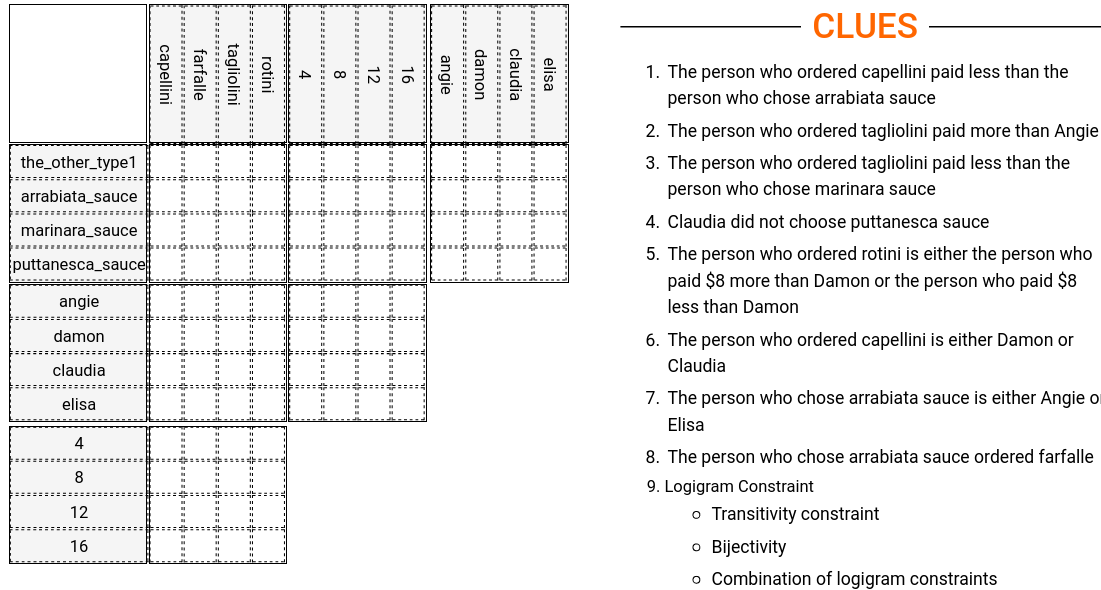
\includegraphics[width=0.9\textwidth]{figures/logic_puzzle.png}
				\vspace{-2mm}
				\caption{\small Logic Grid Puzzle}
			\end{figure}
			\vspace{-6mm}
			\pause
			\begin{figure}[h]
				\centering
				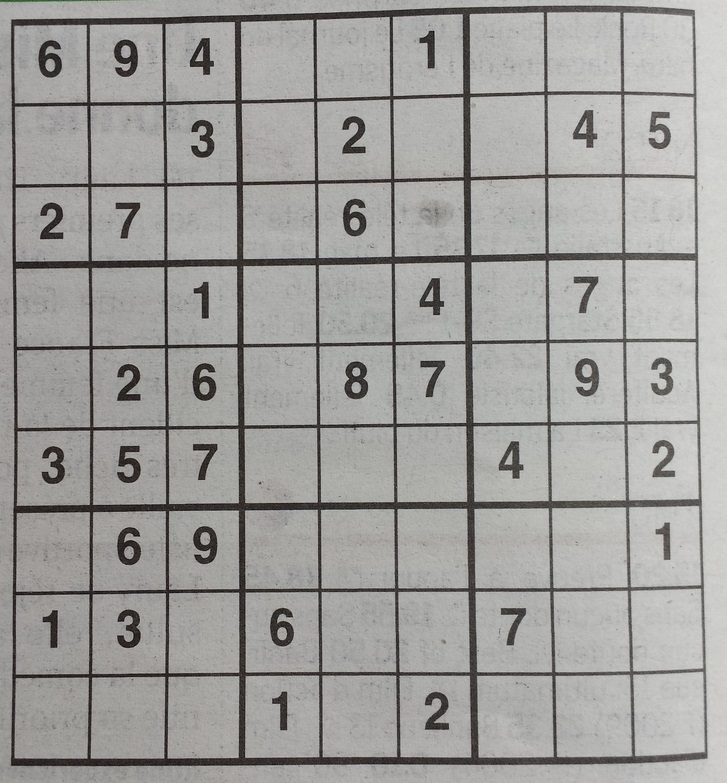
\includegraphics[width=.45\textwidth]{figures/sudoku.jpg}
				\vspace{-2mm}
				\caption{\small Sudoku}
			\end{figure}
		\end{minipage}\pause
		\hfill
		\begin{minipage}[t]{0.45\textwidth}
			\begin{figure}[h]
				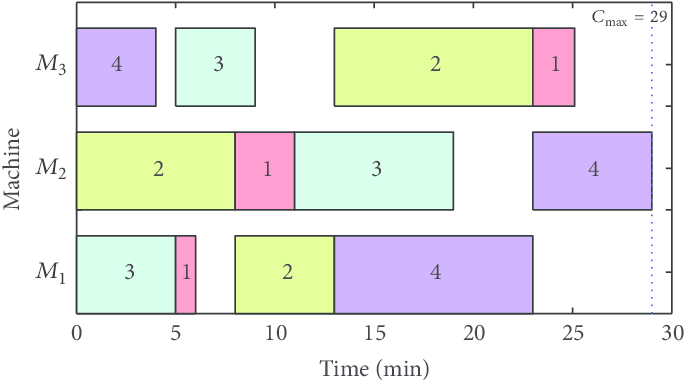
\includegraphics[width=0.9\textwidth]{figures/scheduling.png}
				\vspace{-2mm}
				\caption{\small Scheduling Problem}
			\end{figure}
			\vspace{-6mm}
\pause
			\begin{figure}[h]
				\includegraphics[width=0.9\textwidth]{figures/omus-presentation-car.png}
				\vspace{-2mm}
				\caption{\small Configuration problems}
			\end{figure}
		\end{minipage}
		\footnote{\tiny \url{https://www.researchgate.net/figure/The-schedule-of-4-3-job-shop-scheduling-problem_fig2_301279276}}
	\end{frame}
	
	\begin{frame}
		\begin{center}\Large
			How do you solve a CSP ? 
		\end{center}
		
	\end{frame}
	
	\begin{frame}
				\frametitle{Constraint Satisfaction Problems}
		\framesubtitle{Solving}
%		\framesubtitle{Explaining SAT}

	\begin{center}
		\begin{tikzpicture}[node distance=1.5cm]
					\node (problem) [startstop] {Problem};
					
					\node (model) [startstop, below of=problem] {Model}; 
					\draw [arrow] (problem) -- (model);			
						\node (cpmpy) [right of=model, xshift=1cm] {CPMpy}; 
					\draw [dashed] (model) -- (cpmpy);									
						\pause
					
					\node (solve) [startstop, below of=model] {SOLVE};
					\draw [arrow] (model) -- (solve); \pause
					
					\node  (modelerror) [startstop, below of=solve, xshift=-1.5cm] {\color{red} modeling error?};
					\draw [arrow] (solve) --node[anchor=east,xshift=-0.2cm] {unsat?} (modelerror); \pause
					\node  (solution) [startstop, below of=solve, xshift=1.5cm]  {\color{green} solution};
					%	\node  (solution) [startstop, below of=sat] {\color{green} solution};
					
					\draw [arrow] (solve) --node[anchor=west,xshift=0.2cm] {sat?} (solution);
					
					%	\draw [arrow] (sat) -- (solution);			
					
				\end{tikzpicture}
			\end{center}
	\end{frame}



	
%	\begin{frame}
%		\begin{minipage}{0.44\textwidth}
%			\begin{center}
%\begin{tikzpicture}[node distance=1.5cm]
%	\node (problem) [startstop] {Problem}; 
%	
%	\node (model) [startstop, below of=problem] {Model}; 
%	\draw [arrow] (problem) -- (model);			
%
%	\node (cpmpy) [right of=model, xshift=0.75cm] {CPMpy}; 
%	\draw [dashed] (model) -- (cpmpy);									
%	
%	\node (solve) [startstop, below of=model] {SOLVE};
%	\draw [arrow] (model) -- (solve); 
%	
%	\node  (modelerror) [startstop, below of=solve] {\color{red} modeling error?};
%	\draw [arrow] (solve) --node[anchor=east,xshift=-0.2cm] {unsat?} (modelerror); 
%%	\node  (solution) [startstop, below of=solve, xshift=1.5cm]  {\color{green} solution};
%%%	\node  (solution) [startstop, below of=sat] {\color{green} solution};
%%	
%%	\draw [arrow] (solve) --node[anchor=west,xshift=0.2cm] {sat?} (solution);
%	
%%	\draw [arrow] (sat) -- (solution);			
%	
%\end{tikzpicture}
%\end{center}
%		\end{minipage}
%		\begin{minipage}{0.55\textwidth}
%			Problem Specification 
%				\begin{itemize}
%					\item \textbf{C} Constraints 
%%					\item[Goal] Generate an explanation sequence that explains step-by-step how to derive the facts of the solution.\pause
%				%	\item[$f$] A cost function quantifying explanation difficulty.
%				\end{itemize}
%				
%\textbf{How do you explain UNSAT ? }\pause
%			\begin{itemize}
%				\item Well embedded in literature \pause
%				\item Unsatisfiable cores \pause
%				\item Smallest Unsat core \pause
%				\item Minimum Correction Subsets \pause
%				\end{itemize}
%
%			\end{minipage}
%	\end{frame}

	\begin{frame}
				\frametitle{Motivation}
		\framesubtitle{Explaining SAT problems}
		
			\begin{minipage}{0.44\textwidth}
			\begin{center}
				\begin{tikzpicture}[node distance=1.5cm]
					\node (problem) [startstop] {Problem}; 
					
					\node (model) [startstop, below of=problem] {Model}; 
					\draw [arrow] (problem) -- (model);			
					
					\node (cpmpy) [right of=model, xshift=0.75cm] {CPMpy}; 
					\draw [dashed] (model) -- (cpmpy);									
					
					\node (solve) [startstop, below of=model] {SOLVE};
					\draw [arrow] (model) -- (solve); 
					
%					\node  (modelerror) [startstop, below of=solve] {\color{red} modeling error?};
%					\draw [arrow] (solve) --node[anchor=east,xshift=-0.2cm] {unsat?} (modelerror); 
						\node  (solution) [startstop, below of=solve]  {\color{green} solution};
%						\node  (solution) [startstop, below of=sat] {\color{green} solution};
					%	
						\draw [arrow] (solve) --node[anchor=west,xshift=0.2cm] {sat?} (solution);
					
%						\draw [arrow] (sat) -- (solution);			
					
				\end{tikzpicture}
			\end{center}
		\end{minipage}
		\begin{minipage}{0.55\textwidth}

			\textbf{How do you explain SAT ? }	
		\end{minipage}
					
	\end{frame}



	\section{How to explain CSPs}

			\begin{frame}
	\frametitle{Outline}
	\tableofcontents[currentsection]
\end{frame}
	
	\begin{frame}{Motivation}
		\framesubtitle{Explaining SAT problems}



	\begin{minipage}{0.6\textwidth}
		\begin{problemspec}
	\begin{itemize}
		\item[$\mathbf{C}$] Constraints (alldifferent, ...)
		\item[$\mathbf{I}$] Partial assignment (Givens  in Sudoku) 
		\item[$\mathbf{I_{end}}$] Full assignment
	\end{itemize}
	%					\item[Goal] Generate an explanation sequence that explains step-by-step how to derive the facts of the solution.\pause
	%	\item[$f$] A cost function quantifying explanation difficulty.
\end{problemspec}
	\end{minipage}
	\begin{minipage}{0.39\textwidth}
		\centering
		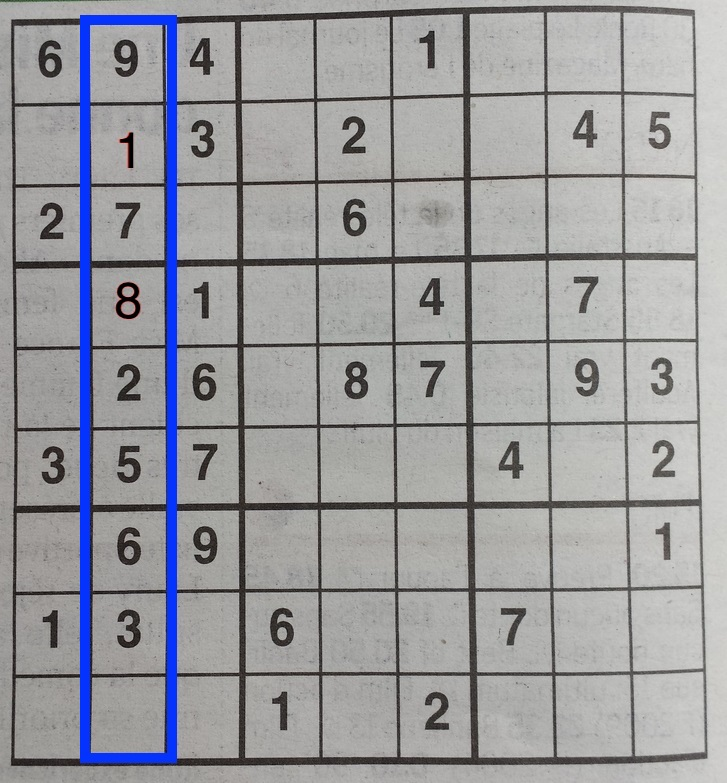
\includegraphics[width=0.6\textwidth]{figures/sudoku_alldiff.jpg}
	\end{minipage}

	\end{frame}


	\begin{frame}{Motivation}
	\framesubtitle{Explaining SAT problems}

\begin{minipage}{0.24\textwidth}	
		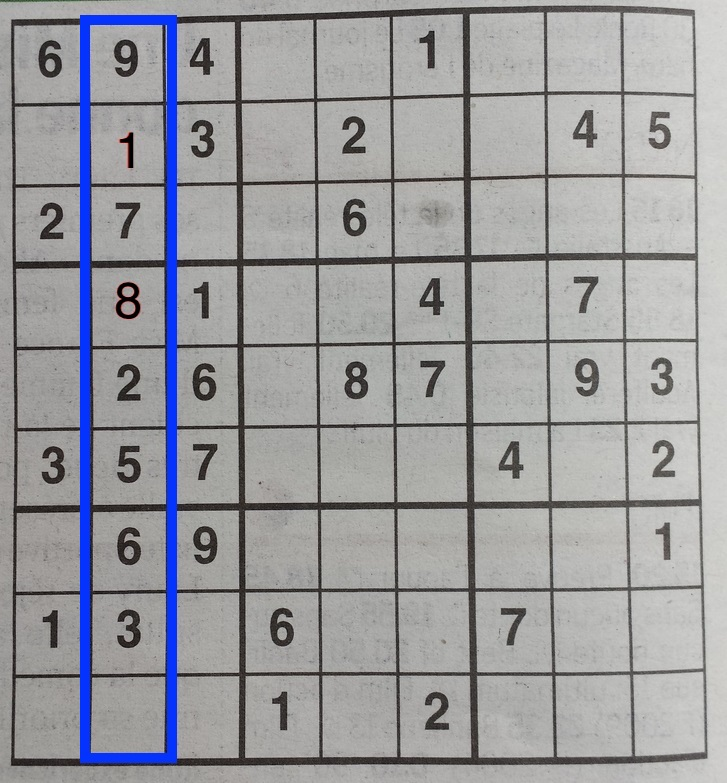
\includegraphics[width=\textwidth]{figures/sudoku_alldiff.jpg}	
\end{minipage}\hfill
\begin{minipage}{0.75\textwidth}
	
	\textbf{How do you explain SAT ? }	\pause
	\begin{itemize}
		\item Sequence of \textit{simple} explanations (\cite{bogaerts2020step})
		
		\item Explanation takes form of a inference step: 
		$ C' \wedge I' \implies N $\pause
		\begin{itemize}
			\item $C' \subseteq \mathbf{C}$ Subset constraints\pause
			\item $I' \subseteq \mathbf{I}$ facts derived\pause
			\item $N  \in \mathbf{sol}\setminus \mathbf{I}$ new fact \pause
		\end{itemize}
		\item $f$ cost function -- quantify explanation difficulty \pause
		\item How to compute them ? \pause
		\begin{itemize}
			\item For every remaining fact-to-explain ($N  \in \mathbf{sol}\setminus \mathbf{I}$) compute 
			\[S = MUS(\mathbf{C} \wedge \mathbf{I} \wedge \lnot N )\]
			\item Select the cheapest one $f(S)$
		\end{itemize}
	\end{itemize}
\end{minipage}



%	\begin{figure}
	%		\includegraphics{imagefile}
	%	\end{figure}
\end{frame}


	\section{Challenges and Open questions}
	
				\begin{frame}
		\frametitle{Outline}
		\tableofcontents[currentsection]
	\end{frame}
	
	
%	\section{Motivation}
	\begin{frame}{Motivation}
		\framesubtitle{Challenges and open questions from \cite{bogaerts2020step}}
		
		\begin{description}[font=\color{vuborange}\itshape]
			%			\small
			\item[Optimality] Explanations not provably optimal, \emph{heuristically} found.
			\begin{itemize}
				\item[$\triangleright$] MUS guarantees non-redundancy but ... not quality.
				%				\item MUS-based heuristic
				\item[$\triangleright$] Alternative: SMUS $\#$-minimal (\cite{ignatiev2015smallest})
			\end{itemize} \pause		
			\item[Efficiency] Explanation generation takes a lot of time: \pause
			\begin{description}
				\item[Constrainedness] Can we avoid looping over the facts when searching for the next best explanation ?\pause
				%					\begin{itemize}
					%						\item[$\triangleright$] \emph{Constrainedness}
					%					\end{itemize}
				\item[Incrementality] Can we reuse information from an explanation call to another?
				%				\begin{itemize}
					%					\item[$\triangleright$] \emph{Incrementality}
					%				\end{itemize}
			\end{description}
		\end{description}
		
	\end{frame}
	
		\section{The OCUS problem}
		
					\begin{frame}
			\frametitle{Outline}
			\tableofcontents[currentsection]
		\end{frame}
		
	
		\begin{frame}
			\frametitle{The OCUS problem}
			\begin{definition}
				\small
				Let $\formula$ be a formula, $f:2^{\formula} \to \nat$ a cost function and  $p$ a predicate $p: 2^{\formula}\to \{\ltrue,\lfalse\}$. We call %a set $U\subseteq \formulag$ a \emph{$p$-constrained $f$-OUS} of \formulag ($(p,f)$-OUS) \tias{what with the OCUS name here?} \bart{I propsoe to say. We call 
					$\subsetT \subseteq \formula$ an \emph{OCUS}$^*$ of \formula (with respect to $f$ and $p$) if \begin{itemize}                                      
						\item $\subsetT$ is unsatisfiable,
						\item $p(\subsetT)$ is true ----- (i.e explain exactly one fact at a time)
						\item \emph{all other unsatisfiable $\subsetT'\subseteq \formula$ with $p(\subsetT')=\ltrue$ satisfy $f(\subsetT')\geq f(\subsetT)$}.
					\end{itemize}
				\end{definition}
				$^*$ = Optimal \emph{Constrained} Unsatisfiable Subset
			\end{frame}
			
			
			

			\begin{frame}{OCUS-Based explanation generation}
				Explanation: 
				$ C' \wedge I' \implies N $
				\begin{itemize}
%					\item $C' \subseteq \mathbf{C}$ Subset constraints
%					\item $I' \subseteq \mathbf{I}$ facts derived
%					\item $N  \in \mathbf{sol}\setminus \mathbf{I}$ new fact \pause
					\item $f$ cost function --- quantify explanation difficutly
					\item $p$ exactly-one($ \{\lnot N  \ : N \in   I_{end} \setminus I \}$) (explain one fact at a time)
				\end{itemize}
					\[\call{OCUS}(C \wedge I  \wedge \{\lnot N : N \in   I_{end} \setminus I \}, f, p)\]

			
				
			\end{frame}
			
			

			
			\section{Results}
						\begin{frame}
				\frametitle{Outline}
				\tableofcontents[currentsection]
			\end{frame}
			
			\begin{frame}{Explanation Quality}

\begin{figure}
	\centering
	\includegraphics[width=0.5\textwidth]{figures/heatmapcosts_ocus_mus_2022040412.pdf}
		\caption{Explanation quality comparison of optimal versus subset-minimal explanations in the generated puzzle explanation sequences.}
	\label{fig:heatmapcostsocusmus2022040412}
\end{figure}
			\end{frame}
						
			\begin{frame}{Incrementality}
				
			\begin{figure}
				\centering
				\includegraphics[width=0.5\textwidth]{figures/incremental_vs_non_SAT_2022_06_01.pdf}
				\caption{Runtime comparison of introducing incrementality on the time to generate a whole explanation sequence with \sat-based \grow.}
				\label{fig:rq2_runtime_incr_non_incr}
			\end{figure}
		
			\end{frame}
			
		
		\section{Conclusion and Future work}
		
					\begin{frame}
			\frametitle{Outline}
			\tableofcontents[currentsection]
		\end{frame}
		
		\begin{frame}{Conclusion}
			In this presentation, we introduce (cost-)\emph{\underline{O}ptimal \underline{C}onstrained} \underline{U}nsatisfiable \underline{S}ubsets (OCUS) to efficiently explain Constraint Satisfaction Problems
			\vfill
			\begin{description}
				\item[Optimality] Cost-function quantifies explanation difficulty. \pause
				\item[Constrainedness] Analyze structural constraints on the form of the explanations. (i.e explain one fact at a time)\pause
				\item[Incrementality] Reuse-information between successive explanation calls.
			\end{description}
			\vfill
		\end{frame}
	
						\begin{frame}
		\frametitle{Outline}
		\tableofcontents[currentsection]
	\end{frame}
	
	\begin{frame}{Conclusion}
		\begin{center}\Large
			What can OCUS do for YOU ? 
		\end{center}
	\begin{figure}
		\centering
		
\includegraphics[width=0.3\textwidth]{figures/i_want_you_ocus.png}
	\end{figure}
	\begin{itemize}
		\item cost-optimal Constrained Unsatisfiable Subsets
		\item Looking for other application domain that can use these 
	\end{itemize}
	\end{frame}
		
		
		\begin{frame}{Future work}
			
			\begin{itemize}
				\item[$\triangleright$] Learning the optimization function (from humans)
				\item[$\triangleright$] Improve the sequence of explanations
				\item[$\triangleright$] Explaining optimization (different types of ``why'' queries);
%				\item[$\triangleright$] Scaling up (approximate algorithms; decomposition of explanation search)
%				\item[$\triangleright$] Incremental algorithms over different ``why'' queries
				% \item 
			\end{itemize}	
			
			
		\end{frame}
		
		
		\begin{frame}
			\begin{center}
				{\huge Questions?}
			\end{center}		
		\end{frame}
		
		
		\begin{frame}[allowframebreaks]
			\frametitle{References}
			\bibliographystyle{named}
			\bibliography{refs}
		\end{frame}
		
		
		
	\end{document}